\chapter*{Exercises C2}

\begin{enumerate}
	\item The frequency table and accompanying cumulative frequency graph are as follows : 
	\begin{table}[h]
		\centering
		\begin{tabular}{@{}ll@{}}
			\toprule
			Value & Frequency \\ \midrule
			3.88  & 3         \\
			3.94  & 2         \\
			3.90  & 2         \\
			3.96  & 2         \\
			3.93  & 2         \\
			3.99  & 1         \\
			3.98  & 1         \\ \bottomrule
		\end{tabular}
	\end{table}
	
	\begin{figure}[!h]
		\centering
		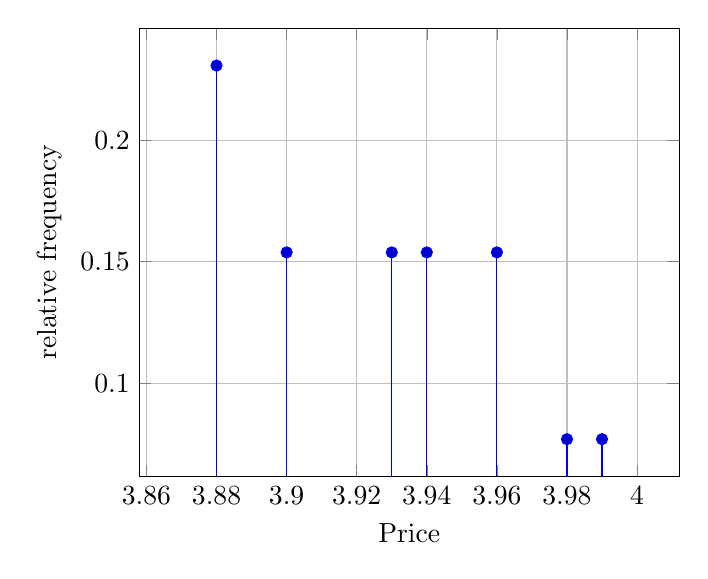
\begin{tikzpicture}
			\begin{axis}[enlarge x limits=0.2, grid = both,
				xlabel = Price, ylabel = relative frequency] 
				\addplot+[ycomb] plot coordinates {(3.88, 3/13) (3.94, 2/13) (3.90, 2/13) (3.96, 2/13) (3.93, 2/13) (3.99, 1/13) (3.98, 1/13)};  
			\end{axis} 
		\end{tikzpicture}
	\end{figure}
	
	\item A pie chart uses the relative frequency of a data entry to allot the sector angle as a proportion of the full 360 degree circle. The sector angle would be $ \theta_i = 360 \times r_i $. \\
	
	\item Pie chart uses the relative frequencies of the 4 entries. \\
	\begin{table}[H]
		\centering
		\begin{tabular}{@{}lll@{}}
			\toprule
			Country       & Oil Reserve & Fraction Oil        \\ \midrule
			United States & 38.7        & 0.30  \\
			South America & 22.6        & 0.17 \\
			Canada        & 8.8         & 0.07  \\
			Mexico        & 60.0        & 0.46  \\ \bottomrule
		\end{tabular}
	\end{table}
	
	\begin{figure}[H]
		\centering
		\caption{Pie chart displaying Oil Reserve percentages}
		\begin{tikzpicture}
			\pie{30/United States,
				17/South Ameruca,
				7/Canada,
				46/Mexico}
		\end{tikzpicture}
	\end{figure}
	
	
	\item The two histograms generated using the first 1000 sentences of two distinct passages are as follows : \\
	
	\begin{figure}[H]
		\centering
		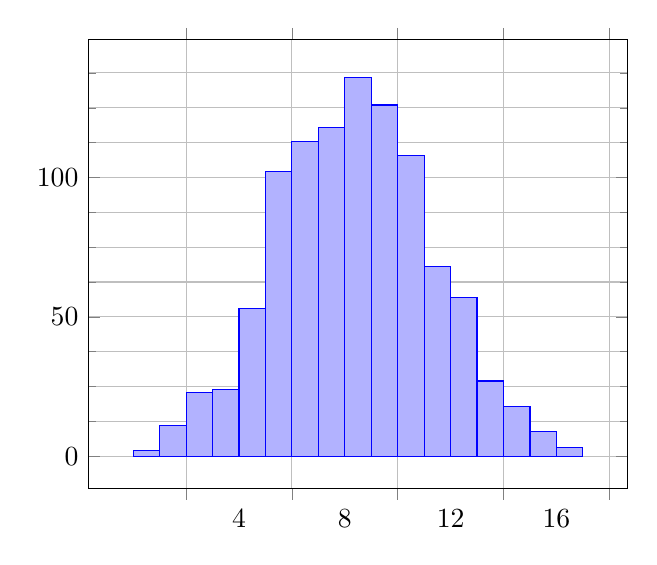
\begin{tikzpicture}
			\begin{axis}[ybar interval, minor y tick num = 3, grid = both, xtick = {0, 4, 8, 12, 16, 20}]
				\addplot coordinates { (2.0, 2)
					(3.0, 11)
					(4.0, 23)
					(5.0, 24)
					(6.0, 53)
					(7.0, 102)
					(8.0, 113)
					(9.0, 118)
					(10.0, 136)
					(11.0, 126)
					(12.0, 108)
					(13.0, 68)
					(14.0, 57)
					(15.0, 27)
					(16.0, 18)
					(17.0, 9)
					(18.0, 3)
					(19.0, 2) };
			\end{axis}
		\end{tikzpicture}
	\end{figure}
	
	
	\begin{figure}[H]
		\centering
		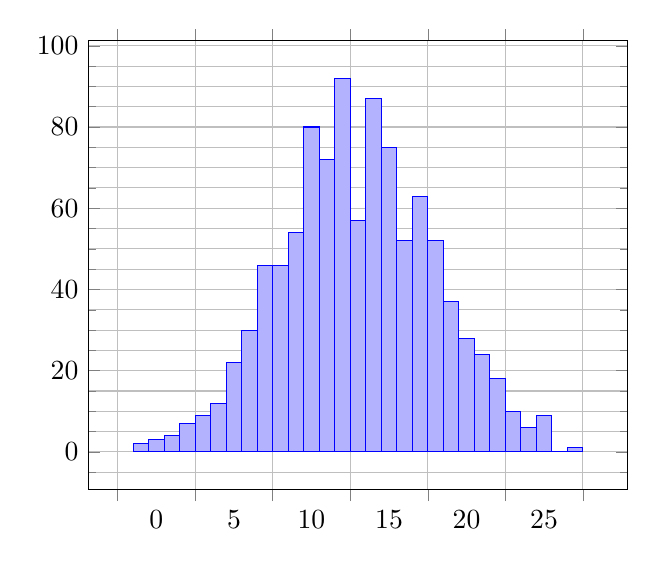
\begin{tikzpicture}
			\begin{axis}[ybar interval, minor y tick num = 3, grid = both, xtick = {0, 5, 10, 15, 20, 25, 30}]
				\addplot coordinates { (1.0, 2)
					(2.0, 3)
					(3.0, 4)
					(4.0, 7)
					(5.0, 9)
					(6.0, 12)
					(7.0, 22)
					(8.0, 30)
					(9.0, 46)
					(10.0, 46)
					(11.0, 54)
					(12.0, 80)
					(13.0, 72)
					(14.0, 92)
					(15.0, 57)
					(16.0, 87)
					(17.0, 75)
					(18.0, 52)
					(19.0, 63)
					(20.0, 52)
					(21.0, 37)
					(22.0, 28)
					(23.0, 24)
					(24.0, 18)
					(25.0, 10)
					(26.0, 6)
					(27.0, 9)
					(28.0, 0)
					(29.0, 1)
					(30.0, 1)};
			\end{axis}
		\end{tikzpicture}
	\end{figure}
	
	No, this would not be sufficient as the distribution always tends to be approximately normal. \\
	
	\item The number of days is the sum of all frequencies $ \sum f_i  = 33$. \\
	The sum of all travel times is the weighted sum of the travel times. $  \sum x_i f_i  = 767 $ \\
	
	\item \begin{enumerate}
		\item The frequency table extracted from the given data is :
		\begin{figure}[H]
			\begin{subfigure}[]{0.45\linewidth}
				\centering
				\begin{table}[H]
					
					\begin{tabular}{@{}rr@{}}
						\toprule
						Accidents & Frequency \\ \midrule
						0         & 1         \\
						1         & 3         \\
						2         & 6         \\
						3         & 4         \\
						4         & 5         \\
						6         & 2         \\
						11        & 1         \\ \bottomrule
					\end{tabular}
				\end{table}
			\end{subfigure}
			%
			\begin{subfigure}[]{0.45\linewidth}
				\centering
				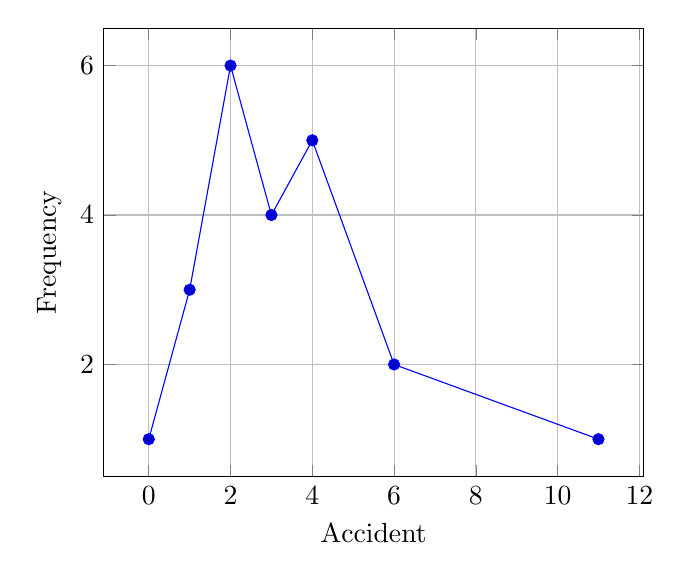
\begin{tikzpicture}
					\begin{axis}[grid = both, xlabel = Accident, ylabel = Frequency]
						\addplot coordinates { (0, 1) (1, 3) (2, 6) (3, 4) (4, 5) (6, 2) (11, 1)};
					\end{axis}
				\end{tikzpicture}
			\end{subfigure}
			
		\end{figure}
		
		\item The frequency polygon is shown above. \\
		
		\item Cumulative relative frequency plot is below \\
		
		\begin{figure}[H]
			\centering
			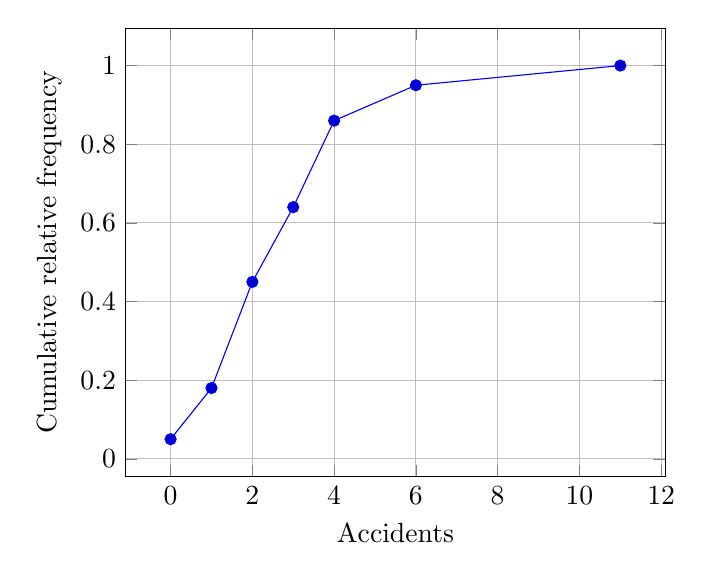
\begin{tikzpicture}
				\begin{axis}[grid = both, xlabel = Accidents, ylabel = Cumulative relative frequency]
					\addplot coordinates {(0, 0.05) (1, 0.18) (2, 0.45) (3, 0.64) (4, 0.86) (6, 0.95) (11, 1.0)};
				\end{axis}
			\end{tikzpicture}
		\end{figure}
		
		\item Mean = 3.18. Median = 3. Mode = 2. Standard Deviation = 2.32.
		
		
	\end{enumerate}
	
	\item \begin{enumerate}
		\item The histogram of fatalities is below. \\
		\begin{figure}[H]
			\centering
			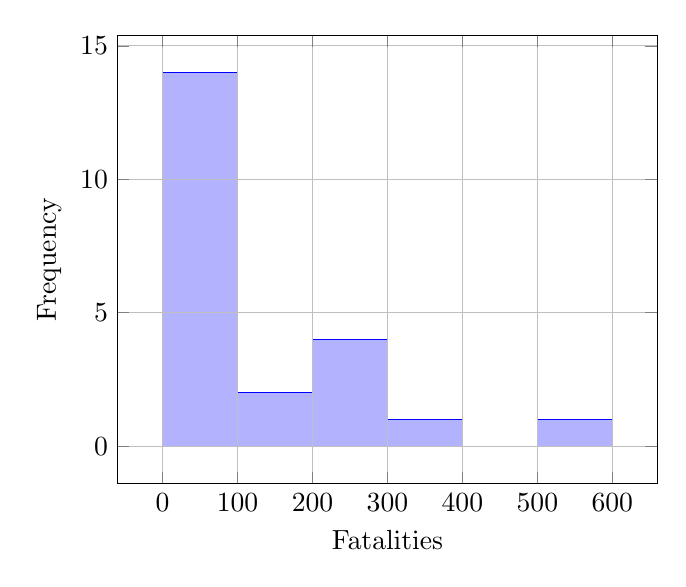
\begin{tikzpicture}
				\begin{axis}[grid = both, xtick = {0, 100, 200, 300, 400, 500, 600, 700}, area style,
					xlabel = Fatalities, ylabel = Frequency]
					\addplot+[ybar interval, mark = no] plot coordinates { (0, 14) (100, 2) (200, 4) (300, 1) (400, 0) (500, 1) (600, 0) };
				\end{axis}
			\end{tikzpicture}
		\end{figure}
		
		\item Stem and leaf plot is just a worse histogram. Ignored.
		\item Mean = 119.14. Median = 3. Mode = 44.5. Standard Deviation = 144.8
	\end{enumerate}
	
	\item Let $ \{x_1\} , \{x_2\} $ be the women and $ \{y_1\} , \{y_2\} $ be the men with means $ \bar{x_1}, \bar{x_2}, \bar{y_1}, \bar{y_2} $ respectively. Given that $ a $ is for all adults,
	\begin{subequations}
		\begin{align}
			\overline{x_1} > \overline{x_2} &\qquad \text{and} \qquad \overline{y_1} > \overline{y_2} \\
			%
			\overline{x_1 + y_1} &= \overline{x_1} + \overline{y_1} \\
			%
			\overline{x_1} + \overline{y_1} &> \overline{x_2} + \overline{y_2} \\
			%
			\overline{x_1 + y_1} &> \overline{x_2 + y_2} \\
			%
			\overline{a_1} &> \overline{a_2}
		\end{align}
		
		The above holds true for real world populations with an almost equal number of men and women. Consider the special case with a fraction $ p $ of the town being male. 
		\begin{align}
			\overline{a_1} &= p_1 \overline{y_1} + (1 - p_1) \overline{x_1} \\
			%
			\overline{a_2} &= p_2 \overline{y_2} + (1 - p_2) \overline{x_2} \\
		\end{align}
		
		It is easy to see that when $ p_1 << p_2 $, but the male and female weight averages are only slightly different between towns A and B, $ a_1 < a_2 $ is possible.
		
	\end{subequations}
	\item Benford's Law in table and graph form : 
	\begin{figure}[H]
		\begin{subfigure}[]{0.45\linewidth}
			\centering
			\begin{table}[H]
				\centering
				\begin{tabular}{@{}rr@{}}
					\toprule
					First digit &  Proportion of data \\
					\midrule
					1 &               0.301 \\
					2 &               0.176 \\
					3 &               0.125 \\
					4 &               0.097 \\
					5 &               0.079 \\
					6 &               0.067 \\
					7 &               0.058 \\
					8 &               0.051 \\
					9 &               0.046 \\
					\bottomrule
				\end{tabular}
			\end{table}
		\end{subfigure}
		%
		\begin{subfigure}[]{0.45\linewidth}
			\centering
			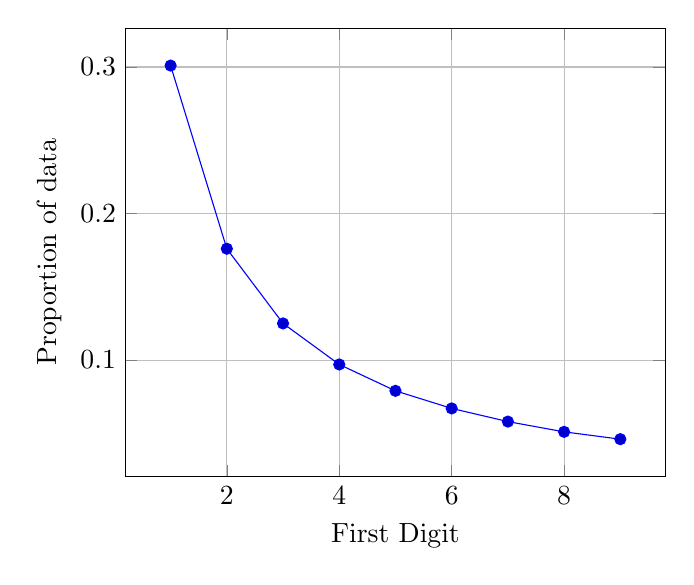
\begin{tikzpicture}
				\begin{axis}[grid = both, xlabel = First Digit, ylabel = Proportion of data]
					\addplot coordinates { (1, 0.301) (2, 0.176) (3, 0.125) (4, 0.097) (5, 0.079) (6, 0.067) (7, 0.058) (8, 0.051) (9, 0.046)};
				\end{axis}
			\end{tikzpicture}
		\end{subfigure} \\		
	\end{figure}
	
	Benford's law would make the option c = 1.4512 the best guess. \\
	
	\item Let the total employee payrolls be $ A_1 $ and $ A_2 $. Then, 
	\begin{subequations}
		\begin{align}
			\overline{x_1} = A_1 / 100 \quad &\text{and} \quad \overline{x_2} = A_2 / 110 \\
			%
			A_1 > A_2 \quad &\implies \quad A_1 / 100 > A_2 / 100 > A_2 / 110 \\
			%
			\overline{x_1} &> \overline{x_2} 
		\end{align}
	\end{subequations}
	
	No comment can be made about the comparison between medians. \\
	
	\item Let the first half dataset be $ \{x_i\} $ and the second half be $ \{y_i\} $, now : 
	\begin{enumerate}
		\item Mean of the first and second half is $\overline{x}$ and $ \overline{y} $, both with same number of elements $ n $. Mean of combined dataset is : 
		\begin{align}
			\overline{z} = \frac{\sum_{i} x_i + \sum_{i} y_i}{n + n} = \frac{\overline{x} + \overline{y}}{2} = 110
		\end{align} \\
		
		\item Median of the combined dataset has to lie between the medians of the first and second halves. $ 100 \leq \text{Median}  \leq 120 $. This assumes that the dataset is sorted before being split into halves. \\
		
		\item No comment can be made about the mode.
	\end{enumerate}
	
	\item Using the midpoints of the class intervals
	\begin{table}[H]
		\centering
		\begin{tabular}{rrrrr}
			\toprule
			StartAge &  EndAge &  Males &  Females &  MidAge \\
			\midrule
			0 &       5 &    120 &       67 &     2.5 \\
			5 &      10 &    184 &      120 &     7.5 \\
			10 &      15 &     44 &       22 &    12.5 \\
			15 &      20 &     24 &       15 &    17.5 \\
			20 &      30 &     23 &       25 &    25.0 \\
			30 &      40 &     50 &       22 &    35.0 \\
			40 &      50 &     60 &       40 &    45.0 \\
			50 &      60 &    102 &       76 &    55.0 \\
			60 &      70 &    167 &      104 &    65.0 \\
			70 &      80 &    150 &       90 &    75.0 \\
			80 &     100 &     49 &       27 &    90.0 \\
			\bottomrule
		\end{tabular}
	\end{table}
	
	\begin{enumerate}
		\item Mean for males = 40.904  and Mean for females = 40.98\\
		\item Median is calculated by finding the class interval containing the middle term and then linearly interpolating within that interval. A similar process is used to find the quartiles. \\
		
		The quartiles for males are 8.3, 47 and 67.3. \\
		The quartiles for females are 8.5, 48.2 and 66.6.
	\end{enumerate}
	
	\item Using the formulas in the text, mean =  15.7, standard deviation = 4.4.
	
	\item Given that $ n = 5 $, $ \overline{x} = 104 $ and $ s^2 = 16 $, 
	
	\begin{subequations}
		\begin{align}
			104 &= \frac{ 102 + 100 + 105 + x_{4} + x_{5} }{5} \\
			%
			x_4 + x_5 &= 213 \\
			%
			16 * (5 - 1) &= (102)^2 + (100)^2 + (105)^2 + (x_4)^2 + (x_5)^2  - (5)(104)^2 \\
			%
			(x_4)^2 + (x_5)^2 &= 22715
		\end{align}
		
		This is a quadratic system of equations with the solution $ x_4 = 110.4 $ and $ x_5 = 102.6 $. \\
	\end{subequations}
	
	\item No. The additional information needed is the population of all the states. This will be used to weight the mean salaries of the individual states to calculate the national average.
	
	\item Mean = 127.425, Std Dev = 11.87, Median = 127.5, Mode = 132.5 (using bin size 5). \\
	The cumulative frequency graph is as follows : 
	
	
	\item Sample mean = 18.9, Median = 19.3, Mode = 21.2, Variance =  6.25\\
	\begin{figure}[H]
		\centering
		
	\end{figure}
	
	\begin{figure}[H]
		\begin{subfigure}[]{0.45\linewidth}
			\centering
			\begin{table}[H]
				\centering
				\begin{tabular}{rr}
					\toprule
					Midpoints &  Frequency \\
					\midrule
					13.5 &          2 \\
					14.5 &          2 \\
					15.5 &          3 \\
					16.5 &          4 \\
					17.5 &          6 \\
					18.5 &          7 \\
					19.5 &          6 \\
					20.5 &         10 \\
					21.5 &          5 \\
					22.5 &          1 \\
					23.5 &          4 \\
					\bottomrule
				\end{tabular}
			\end{table}
		\end{subfigure}
		%
		\begin{subfigure}[]{0.45\linewidth}
			\centering
			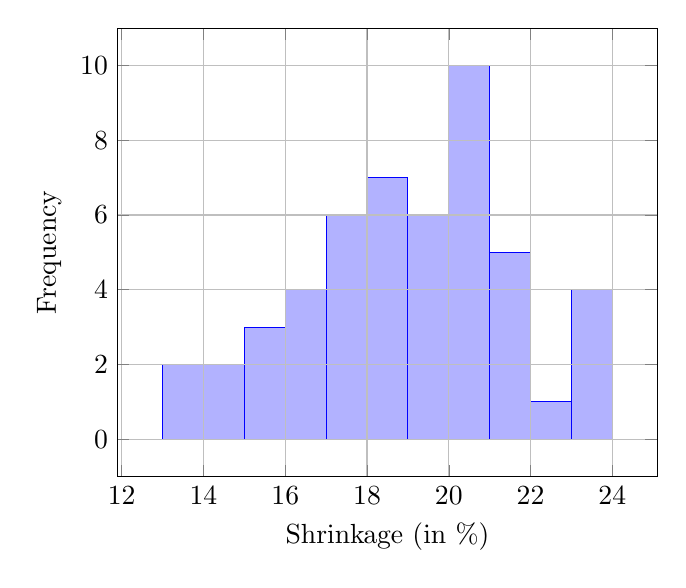
\begin{tikzpicture}
				\begin{axis}[grid = both, xlabel = Shrinkage (in \%), ylabel = Frequency, area style]
					\addplot+[ybar interval, mark = no] plot coordinates {(13, 2) (14, 2) (15, 3) (16, 4) (17, 6) (18, 7) (19, 6) (20, 10) (21, 5) (22, 1) (23, 4) (24, 0)};
				\end{axis}
			\end{tikzpicture}
		\end{subfigure} \\		
	\end{figure}
	
	Using the table with midpoints above, Mean = 18.98, Variance = 6.53. They differ from the actual mean and variance above because of the binning approximations.
	
	\item The recursive mean formula can be proved using : 
	
	\begin{subequations}
		\begin{align}
			\overline{x}_{j + 1} &= \frac{1}{j + 1} \sum\limits_{i = 1}^{j + 1} x_{i} \\
			%
			& = \frac{j}{j + 1} \left( \frac{1}{j} \sum\limits_{i = 1}^{j} x_{i} \right) + \frac{x_{j + 1}}{j + 1} \\
			%
			& = \left( 1 - \frac{1}{j + 1} \right) \overline{x}_{j} + \frac{x_{j + 1}}{j + 1} \\
			%
			& = \overline{x}_{j} + \frac{x_{j + 1} - \overline{x}_{j}}{j + 1}
		\end{align}
	\end{subequations} \\
	
	Using the normal method, mean = 5.16 and variance = 6.96. \\
	Using the recursive formula, mean = 5.16 and variance = 6.96. They match. \\
	
	\item The 90 percentile for January averages is 46 degrees. \\
	The 75 percentile for January averages is 70.45 degrees.
	
	\item The quartiles are 74, 85, 91.5.\\
	
	\item Mean = 84.92, variance = 928.63. \\
	Quartiles are 60.25, 95.5, 113.25. \\
	
	\item ... larger than all of the existing values. \\
	
	\item The box plot representing the data is as follows : \\
	
	\begin{figure}[H]
		\centering
		\begin{tikzpicture}
			\begin{axis}[
				y=2in,
				]
				\addplot+ [
				boxplot prepared={
					lower whisker=60,
					lower quartile=74,
					median=85,
					upper quartile=91.5,
					upper whisker=98,
				},
				]
				table [row sep=\\,y index=0] {
					data\\
				};
			\end{axis}
		\end{tikzpicture}
	\end{figure}
	
	\item The data is shown as a histogram as follows. It is not a normal distribution. \\
	
	\begin{figure}[H]
		\centering
		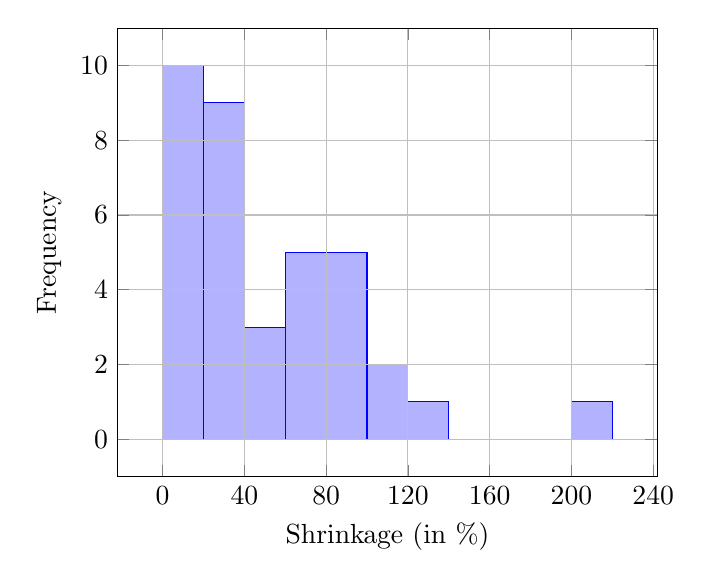
\begin{tikzpicture}
			\begin{axis}[grid = both, xlabel = Shrinkage (in \%), ylabel = Frequency, area style,
				xtick = { 0,  40,  80, 120, 160, 200, 240}]
				\addplot+[ybar interval, mark = no] plot coordinates { (0, 10) (20, 9) (40, 3) (60, 5) (80, 5) (100, 2) (120, 1) (140, 0) (160, 0) (180, 0) (200, 1) (220, 0) };
			\end{axis}
		\end{tikzpicture}
	\end{figure} 
	
	
	\item Mean = 0.35, Median = 0.35, Standard Deviation = 0.117, with the histogram looking approximately normal. \\
	37 of 55 values (67 \%) are within 1 std of the mean. \\
	
	\begin{figure}[H]
		\centering
		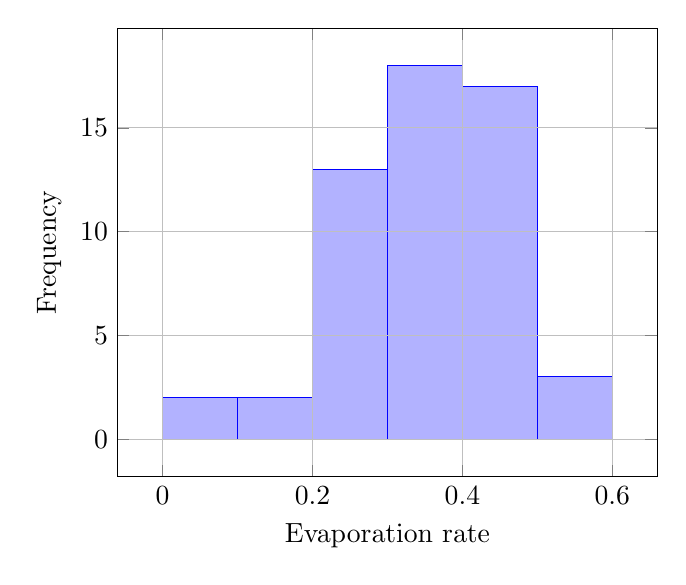
\begin{tikzpicture}
			\begin{axis}[grid = both, xlabel = Evaporation rate, ylabel = Frequency, area style,
				xtick = {0, 0.2, 0.4, 0.6, 0.8}]
				\addplot+[ybar interval, mark = no] plot coordinates { (0.0, 2) (0.1, 2) (0.2, 13) (0.3, 18) (0.4, 17) (0.5, 3) (0.6, 0)};
			\end{axis}
		\end{tikzpicture}
	\end{figure} 
	
	\item \begin{enumerate}
		\item Mean = 3.72, std dev = 0.146. \\
		
		
		\item 80\% of entries are within 1.5 std dev of the mean. Chebyshev inequality lower limit is 55.6 \%. \\
		\item 100\% of entries are within 2 std dev of the mean. Chebyshev inequality lower limit is 75 \%. \\
		\item Stem and leaf plot is replaced by histogram here.
		
		\begin{figure}[H]
			\centering
			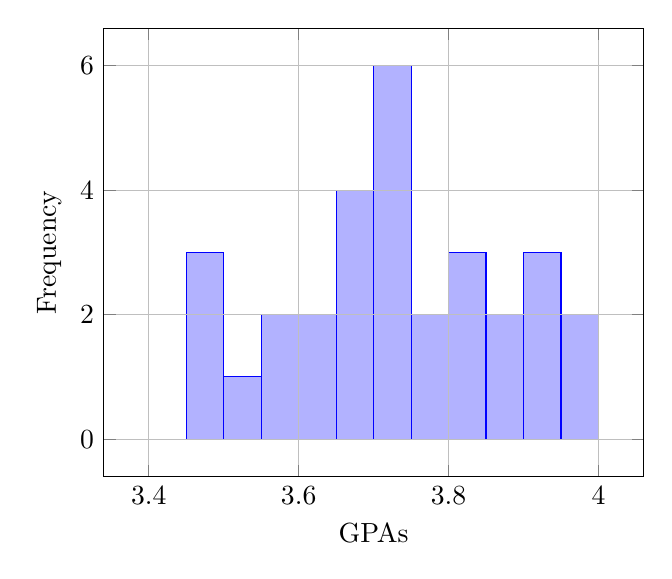
\begin{tikzpicture}
				\begin{axis}[grid = both, xlabel = GPAs, ylabel = Frequency, area style,
					xtick = {3.2, 3.4, 3.6, 3.8, 4.0, 4.2}]
					\addplot+[ybar interval, mark = no] plot coordinates { (3.4, 0) (3.45, 3) (3.5, 1) (3.55, 2) (3.6, 2) (3.65, 4) (3.7, 6) (3.75, 2) (3.8, 3) (3.85, 2) (3.9, 3) (3.95, 2) (4.0, 0)};
				\end{axis}
			\end{tikzpicture}
		\end{figure} 
		
		
	\end{enumerate}
	
	\item The approximate Chebyshev limits do not match the actual proportions. This is because the dataset is not normally distributed. \\
	
	The empirical value numbers are calculated using the area under the curve of a standard normal distribution in the interval [$ -k, k $] in order to find the fraction of data points in the interval [$ \mu - k \sigma, \mu + k \sigma $] \\
	
	The empirical rule dictates that the fraction of data points within 1.5 std dev of the mean is 86.6 \%, compared to observed value of 80 \% \\
	The empirical rule dictates that the fraction of data points within 2 std dev of the mean is 95 \%, compared to observed value of 100 \% \\
	
	\item No, because the health club consists of members of the total population who are above average weight. 
	
	\item \begin{enumerate}
		\item Mean = 127.425, Median = 127.5. \\
		
		\item A histogram of the data to check if it is normal : yes it is. \\
		
		\begin{figure}[H]
			\centering
			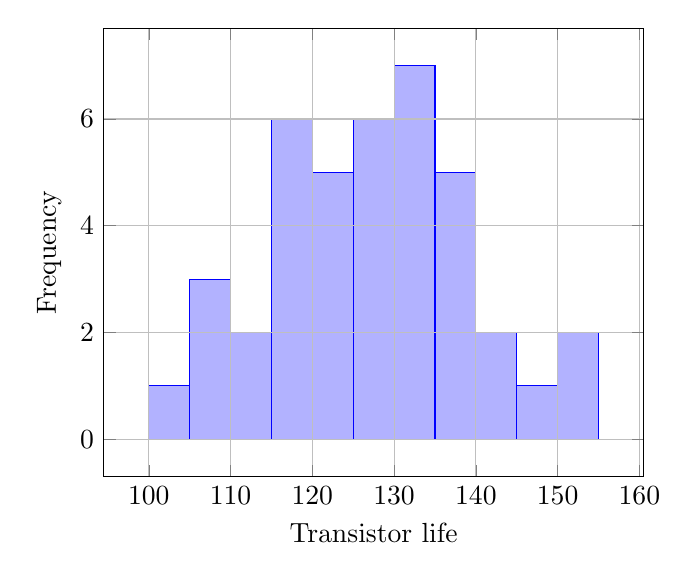
\begin{tikzpicture}
				\begin{axis}[grid = both, xlabel = Transistor life, ylabel = Frequency, area style]
					\addplot+[ybar interval, mark = no] plot coordinates {(100, 1) (105, 3) (110, 2) (115, 6) (120, 5) (125, 6) (130, 7) (135, 5) (140, 2) (145, 1) (150, 2) (155, 0)};
				\end{axis}
			\end{tikzpicture}
		\end{figure} 
		
		\item Standard Deviation = 11.87. \\
		
		\item The empirical rule dictates that the fraction of data points within 1.5 std dev of the mean is 86.6 \%, compared to observed value of 85 \%. \\
		
		\item The Chebyshev minimum fraction is 55.6 \% of data within 1.5 std dev of the mean. This rule is obeyed. \\
	\end{enumerate}
	
	\item Sample correlation coefficient is r = 0.484 \\
	
	\begin{figure}[H]
		\centering
		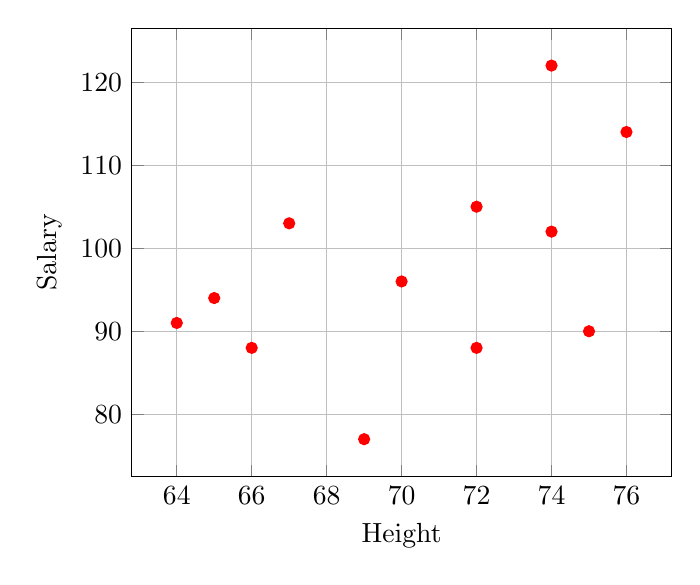
\begin{tikzpicture}
			\begin{axis}[grid = both, xlabel = Height, ylabel = Salary]
				\addplot[only marks, color = red] coordinates {(64, 91) (65, 94) (66, 88) (67, 103) (69, 77) (70, 96) (72, 105) (72, 88) (74, 122) (74, 102) (75, 90) (76, 114)
				};
			\end{axis}
		\end{tikzpicture}
	\end{figure}
	
	\item No causation can be declared from the correlation. It is possible that the good posture is a result of trying to relieve the back pain. \\
	
	\item No. A possible explanation is that immigrants tend to settle down in higher-paying states. \\
	
	\item r = 0.743 between Hours studied and GPA. \\
	
	\item 	Verifying property 3 of sample correlation coefficient : 
	
	\begin{subequations}
		\begin{align}
			y_i \ &=\  a + b x_i \qquad \text{with} \qquad b < 0 \\
			%
			s_{y}^{2} \ &=\ b^2 s_{x}^2 \\
			%
			r \ &=\ \frac{\sum_{i} (x_i - \bar{x}) (y_i - \bar{y})}{(n - 1) s_x s_y} \\
			%
			r \ &=\ \frac{b \sum_{i} (x_i - \bar{x})^{2}}{- b (n - 1) s_{x}^{2}} \\
			%
			r &= -1			
		\end{align}
	\end{subequations}\\
	
	\item Verifying property 4 : 
	
	\begin{subequations}
		\begin{align}
			p_i \ &=\  a + b x_i \qquad q_i \ =\  c + d y_i \qquad \text{with} \qquad bd > 0 \\
			%
			s_{p}^{2} \ &=\ b^2 s_{x}^2 \qquad \text{and} \qquad s_{q}^{2} \ =\ d^2 s_{y}^2 \\
			%
			r_{pq} \ &=\ \frac{\sum_{i} (p_i - \bar{p}) (q_i - \bar{q})}{(n - 1) s_p s_q} \\
			%
			r_{pq} \ &=\ \frac{bd \sum_{i} (x_i - \bar{x}) (y_i - \bar{y})}{|bd| (n - 1) s_{x} s_{y}} \\
			%
			r_{pq} &= r_{xy} \qquad \text{if} \qquad bd > 0			
		\end{align}
	\end{subequations}\\
	
	\item Grades 2-4 imply children with a range of ages, so height is less likely to be directly causing the higher reading scores  compared to age itself. \\
	
	\item Family wealth, nurture and the emphasis it places on early literacy, school environments and peer group are all possible confounding factors that are extremely difficult to adjust for. \\
	
	\item The Lorenz curve is as follows, with Gini Index = 0.1567.
	
	\begin{figure}[H]
		\centering
		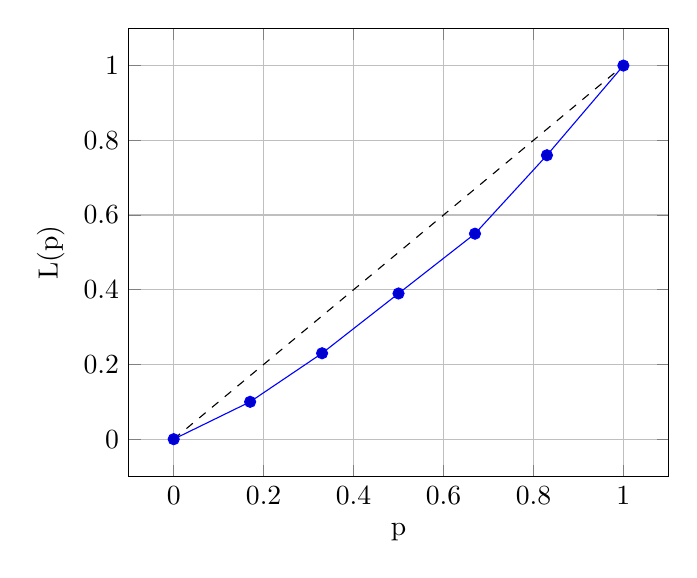
\begin{tikzpicture}
			\begin{axis}[grid = both, xlabel = p, ylabel = L(p)]
				\addplot coordinates {(0.0, 0.0) (0.17, 0.1) (0.33, 0.23) (0.5, 0.39) (0.67, 0.55) (0.83, 0.76) (1.0, 1.0)
				};
				\draw[dashed] (axis cs:0, 0) -- (axis cs:1, 1);
			\end{axis}
			
		\end{tikzpicture}
	\end{figure} 
	
	\item The Lorenz curve is as follows, with Gini Index = 0.163. \\
	
	\begin{figure}[H]
		\centering
		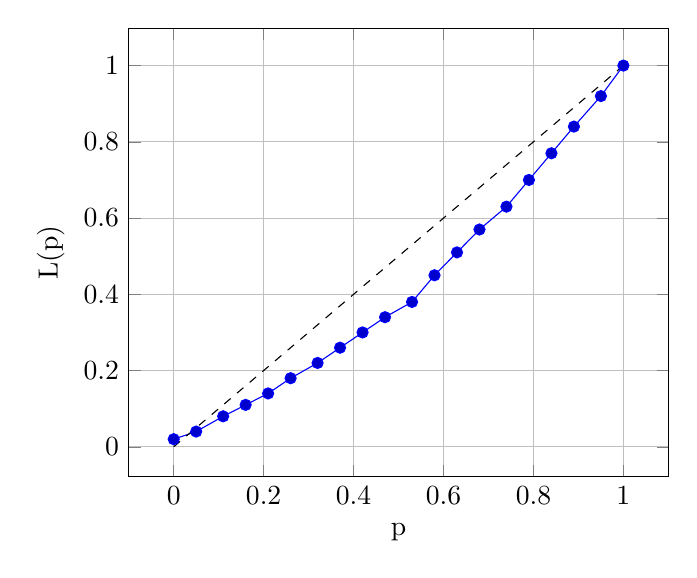
\begin{tikzpicture}
			\begin{axis}[grid = both, xlabel = p, ylabel = L(p)]
				\addplot coordinates {(0.0, 0.02) (0.05, 0.04) (0.11, 0.08) (0.16, 0.11) (0.21, 0.14) (0.26, 0.18) (0.32, 0.22) (0.37, 0.26) (0.42, 0.3) (0.47, 0.34) (0.53, 0.38) (0.58, 0.45) (0.63, 0.51) (0.68, 0.57) (0.74, 0.63) (0.79, 0.7) (0.84, 0.77) (0.89, 0.84) (0.95, 0.92) (1.0, 1.0)
				};
				\draw[dashed] (axis cs:0, 0) -- (axis cs:1, 1);
			\end{axis}
			
		\end{tikzpicture}
	\end{figure} 
	
	\item From the formula for the Lorenz curve data points, multiplying all data by a constant has no effect as it cancels out. \\
	Adding a positive constant to every data point, makes some Lorenz values larger and some smaller. So, the effect on the Gini index cannot be predicted. \\
	
\end{enumerate}

